% THE EXPERIMENTAL DESIGN. Two conditions crossed with five tasks, within
% dyads, drawn as a grid so a reader can count the cells. The rejected
% alternatives are a table beneath rather than a box beside, so the figure
% fits the text column at full size.
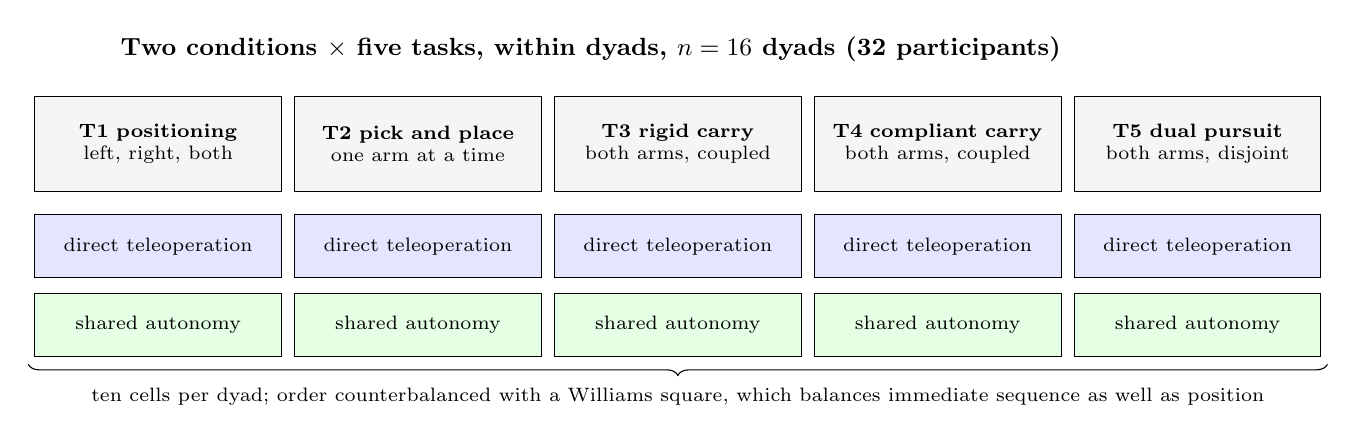
\begin{tikzpicture}[x=1mm, y=1mm, font=\scriptsize]

\node[font=\bfseries\small, anchor=west] at (-6, 12)
  {Two conditions $\times$ five tasks, within dyads, $n = 16$ dyads (32 participants)};

\foreach \i/\t/\n in {0/{T1 positioning}/{left, right, both},
                      1/{T2 pick and place}/{one arm at a time},
                      2/{T3 rigid carry}/{both arms, coupled},
                      3/{T4 compliant carry}/{both arms, coupled},
                      4/{T5 dual pursuit}/{both arms, disjoint}}
{
  \pgfmathsetmacro{\x}{\i*33}
  \node[draw, fill=gray!8, minimum width=31mm, minimum height=12mm,
        align=center, text width=29mm] at (\x, 0) {\textbf{\t}\\\n};
  \node[draw, fill=blue!10, minimum width=31mm, minimum height=8mm,
        align=center, text width=29mm] at (\x, -13) {direct teleoperation};
  \node[draw, fill=green!10, minimum width=31mm, minimum height=8mm,
        align=center, text width=29mm] at (\x, -23) {shared autonomy};
}
\draw[decorate, decoration={brace, mirror, amplitude=4pt}]
  (-16.5, -28) -- (148.5, -28)
  node[midway, below=5pt, font=\scriptsize]
  {ten cells per dyad; order counterbalanced with a Williams square, which
   balances immediate sequence as well as position};
\end{tikzpicture}
